\documentclass{article}

\usepackage{graphicx}
\usepackage{cleveref}

\begin{document}

\title{Project in Advanced Multiprocessor Programming - Concurrent Bags}
\author{Christian Sallinger - 11805799}
\maketitle

\section{Introduction}

In our project we were dealing with a lock-free algorithm for concurrent bags as proposed by Håkan Sundell, Anders Gidenstam, Marina Papatri-
antafilou and Philippas Tsigas. 


\section{The algorithm}

The main idea of the algorithm is to use thread-local storage (TLS) to store items added to the bag as well as some meta information.
To remove an item, each thread first tries to return an item from its own TLS. If the thread does not hold any items in its TLS it tries to steal
from one of the other threads, removing an item from their TLS.

To be more precise, each thread stores items in a linked list of blocks, where each block itself can hold a fixed size of items. Also in TLS is the current position
for adding and removing items, called the threadHead in the paper. There is also a pointer to the first block in the linked list of blocks, called the threadBlock. For the 
purpose of trying to steal elements the threads also store the last tried position of a steal and a pointer to the last block where stealing was tried.

The removal of items from any of the blocks is the critical step where we have to ensure that the item was not already returned by another thread. To ensure the removal of the item
happens only once the Compare-And-Swap (CAS) atomic synchronization primitive is used.


Here goes your report with plots as beautiful as \cref{fig:example_plot}.

\begin{figure}[ht!]
  \centering
  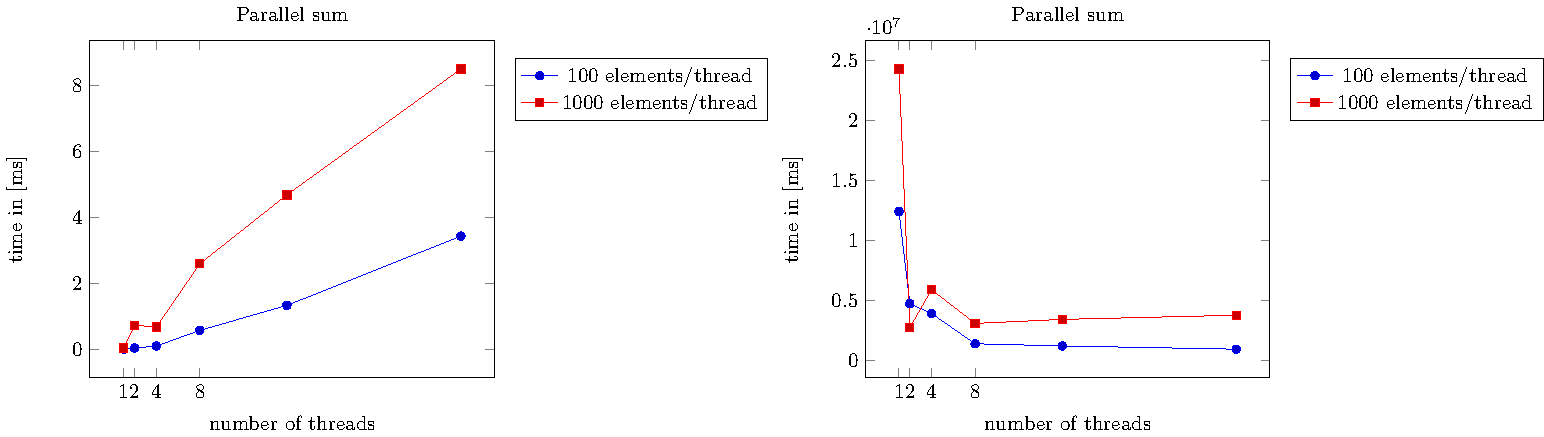
\includegraphics[width = \textwidth]{../plots/avg_plot.pdf}
  \caption{A sample plot showcasing the runtime of a distributed library under
  increasing number of threads. Clearly, it does not scale very well.}
  \label{fig:example_plot}
\end{figure}

\end{document}
